\documentclass[11pt,letterpaper]{article}
\usepackage[utf8]{inputenc}
\usepackage[margin=1in]{geometry}
\usepackage[margin=1cm]{caption}
\usepackage{amsmath}
\usepackage{amsfonts}
\usepackage{amssymb}
\usepackage{amsthm}
\usepackage{verbatim}
\usepackage{graphicx}
\usepackage{sidecap}
% No paragraph tabs
\setlength{\parindent}{0pt}

% Define commands that will be widely used.
\newcommand{\br}{\ \\}
\newcommand{\tab}{\hspace*{2em}}

\title{Brownian Motion in Cells}
\author{Rachel Domagalski\\
Partner: Matthew Turner}
\date{December 16, 2013}

\begin{document}
\maketitle

\begin{abstract}
    The diffusion of a particle in a solvent can be described by Einstein's
    theory of Brownian motion. In this theory, the displacements of particles
    are Gaussian distributed and the diffusion coefficient of the system can be
    computed from the mean-square of the displacements of particles in the
    system. The theory of Brownian motion can be applied to the motion of
    vesicles in cells. However, diffusion is insufficient to explain the
    transport of vesicles in cells and active transport methods are required to
    explain the transport.
\end{abstract}

\section{Introduction}

% OUTLINE
% 1. Talk about what brownian motion is and how it was disovered.
% 2. Give a brief mathematical description of the brownian motion.
% 3. Talk about brownian motion in cells.
% 4. Briefly describe the experiment.

In 1827, the when the botanist Robert Brown was studying pollen grains suspended
in water, he noticed that small particles were being expelled from the grains
\cite{BMWikipedia}. These small particles, suspended in the water, had a random
motion, and Brown was unable to determine the cause of their motion. That random
and jittery motion and diffusion of the particles later became known as Brownian
motion and its cause was explained in great detail by Albert Einstein
\cite{EinsteinBrownian}. In 1908, the experimentalist Jean Perrin confirmed that
Einstein's theory of Brownian motion was correct, earning him a Nobel Prize in
physics in 1926.\\

In his 1905 paper, Einstein showed that the displacements of particles from
their origins follows the diffusion equation
\begin{equation}
    \frac{\partial f}{\partial t} = D \frac{\partial^2 f}{\partial x^2}
    \label{diffusioneq}
\end{equation}
where $D$ is the diffusion coefficient \cite{EinsteinBrownian}. When using the
conditions that lead to Brownian motion, \eqref{diffusioneq} has the solution
\begin{equation}
    f\left(x, t\right) = \frac{1}{\sqrt{4\pi Dt}} e^{-\frac{x^2}{4Dt}}
    \label{desolution}
\end{equation}
This distribution is Gaussian, so it has a mean of 0 and variance of $2Dt$.
Since the mean of the Gaussian in \eqref{desolution} is zero, $\sigma^2 =
\langle x^2 \rangle = 2Dt$ in this case. These mathematical facts about the
behavior of Brownian motion will come in handy when constructing simulations and
when investigating diffusion.\\

Brownian motion is useful in explaining certain cellular behavior, and Brownian
motion is something that can be measured when observing cells. Two examples of
cellular objects that undergo Brownian motion are vesicles and mitochondria. The
diffusion through Brownian motion in cells is a passive method of transporting
material from one location to another. However, many cellular transport
processes are more directed and deterministic, and Brownian motion simply is not
enough to explain cellular transport. In addition to the passive transport
method of diffusion, cells also use active transport methods to move material,
and these active transport methods can be measured using the same experimental
techniques used to measure Brownian motion.

\section{Simulating Brownian Motion}

% OUTLINE
% 1. Quick intro.
% 2. Diffusion simulations
% 3. Bulk flow simulations

Brownian motion experiments can be simulated on a computer with Monte Carlo
simulations. This is useful because the simulations demonstrate what to expect
when taking measurements on a system with certain conditions. In Brownian
motion, the total displacement of a particle is the sum of tiny displacements of
the particle from its origin. The distribution of these tiny displacements is
given by \eqref{desolution}, and this makes creating Monte Carlo simulations
Brownian motion very straightforward to implement.

\subsection{The Diffusion Coefficient}

The goal of the Monte Carlo is to generate random particle trajectories and use
them to compute the diffusion coefficient. The mean-square displacements can be
related to the diffusion coefficient since \cite{LabManual}
\begin{equation}
    \langle \left| \vec{r}\left(t + \Delta t\right) -
    \vec{r}\left(t\right) \right|^2 \rangle = 2dD\Delta t
    \label{diffusion_data}
\end{equation}
where $d$ is the number of dimensions in the simulation. Each component of
displacement in the particle's trajectory is taken by sampling from a normal
distribution where $\sigma^2 = 2 D \Delta t$. This variance comes from the
Gaussian described in \eqref{desolution}, and this determines the length scale
of the simulation. The theoretical value of diffusion is \cite{LabSim}
\begin{equation}
    D = \frac{k_B T}{3\pi\eta r}
    \label{diffusion_def}
\end{equation}
where $k_B$ is Boltzmann's constant, $T$ is the temperature of the solution,
$\eta$ is the viscosity of the solution, and $r$ is the radius of the particles
in the solution. This value of the diffusion coefficient is that can be used to
sample the displacements of the particles.\\

% Basic brownian motion simulation with one particle track.
\begin{figure}
    \centering
    \begin{minipage}[t]{0.485\textwidth}
        \centering
        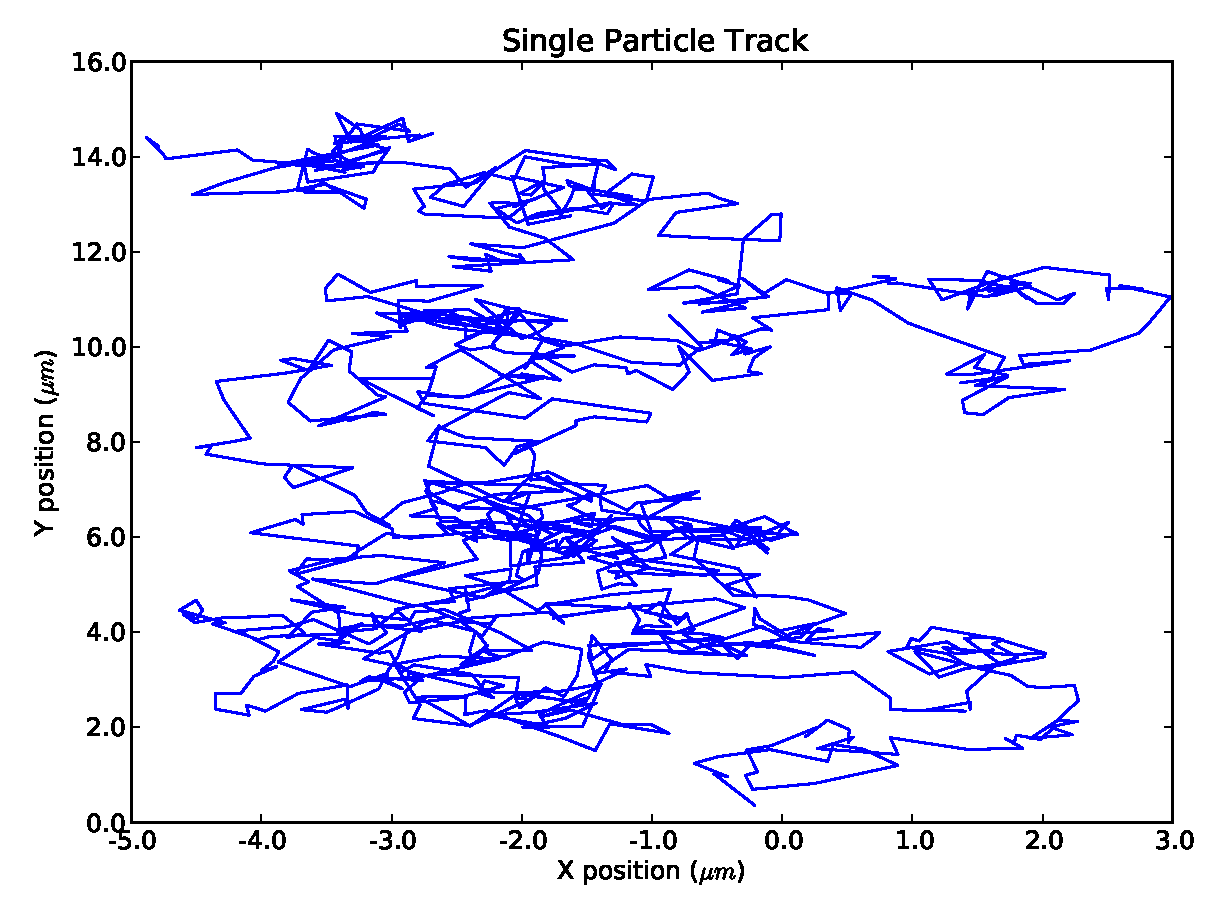
\includegraphics[width=\textwidth]{figures/brownian_track.pdf}
    \end{minipage}
    \begin{minipage}[t]{0.485\textwidth}
        \centering
        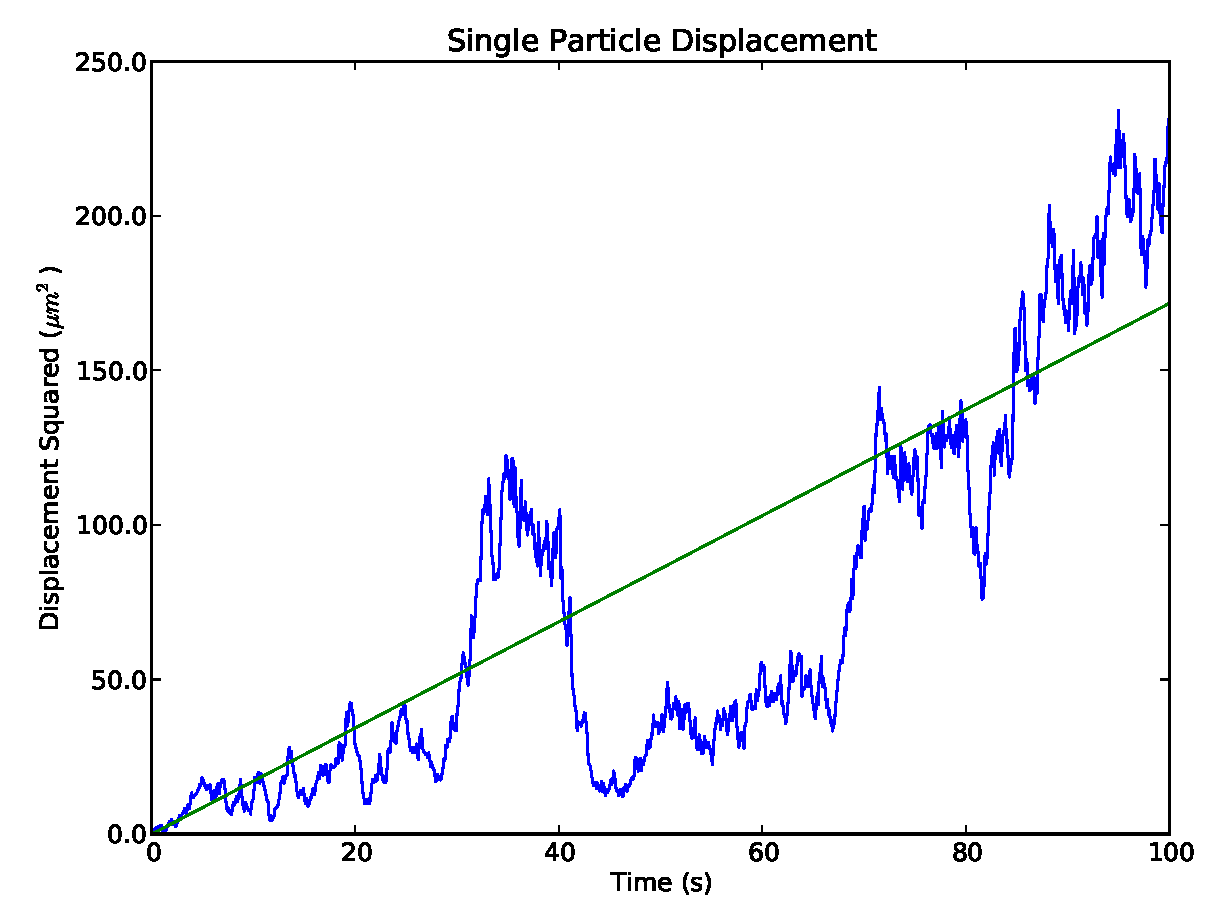
\includegraphics[width=\textwidth]{figures/brownian_dispsq.pdf}
    \end{minipage}
    \caption{Monte Carlo simulation for a system with a diffusion coefficient of
        \mbox{0.429 $\mu m^2 / s$}. The measured diffusion coefficient for this
        simulation was \mbox{$0.427 \pm 1.6 \times 10^{-3} \mu m^2 / s$}. The
        particle for this simulation had a radius of $1 \mu m$ and the viscosity
        of the simulation was 1 cP. The temperature of the solution was 20
        $^\circ \text{C}$ and displacement measurements were taken every 0.1
        seconds.}
    \label{brownian_sim}
\end{figure}

At a first glance, the description of the simulation might seem kind of
circular. In order to measure the diffusion coefficient from a random sampling,
one needs to know what the diffusion coefficient is. The point of the Monte
Carlo simulation is to get measurements of the diffusion coefficient from
particle tracks and to determine how long a particle track needs to be in order
to get a certain precision. A quick example of a Monte Carlo simulation for a
one-particle system with particles of radius of 1 $\mu m$ in solution with
viscosity of 1 cP can be seen in Figure~\ref{brownian_sim}. Another simulation
that can be done is a system with many particles (see
Figure~\ref{many_particles_sim}). This simulation is useful because it matches
what will me measured in an actual experiment much more closely than the
one-particle simulation. The reasons for this is that in an actual experiment,
multiple particles will be tracked. Additionally, the particles in an experiment
will only be tracked for about 10 to 50 displacements. In a one-particle system,
that would not give a very precise value of diffusion. However, adding more
particles to the system makes the measured value of diffusion much more
precise.\\

% Talk about how many particles are needed to get a certain level of precision.
% TODO figure out what the theoretical error should be.
It is important to check how many steps in a particle track is needed to get a
certain level of precision. Since the diffusion coefficient is obtained from
$\langle \Delta r^2 \rangle$, the variance of $\Delta x^2$ can be computed as
\begin{equation}
    \sigma_{\Delta x^2} = \sqrt{
    \langle \Delta x^4 \rangle -
    \langle \Delta x^2 \rangle^2 }
    = 2 \sqrt{2} D \Delta t
\end{equation}
It can be seen from the fact that since
$\displaystyle D = \frac{\langle \Delta x^2 \rangle}{2 \Delta t}$, the error for
computing $D$ by averaging $\Delta r^2$ should be
\begin{equation}
    \sigma_D = D \sqrt{\frac{2}{dnN}}
\end{equation}
where $d$ is the number of dimensions, $n$ is the number of tracks, and $N$ is
the number of particles in the system. This theoretical value of the uncertainty
can be used to show that if one wants a precision of 1\% on the value of the
diffusion coefficient for a 2-dimensional system, then one would need to track
one particle for 10,000 steps. Alternatively, the same precision could be
achieved by tracking 100 particles for 100 steps each or any other combination
of $n$ and $N$ where $nN = 10,000$.

% Combined particle tracks.
\begin{figure}
    \centering
    \begin{minipage}[t]{0.485\textwidth}
        \centering
        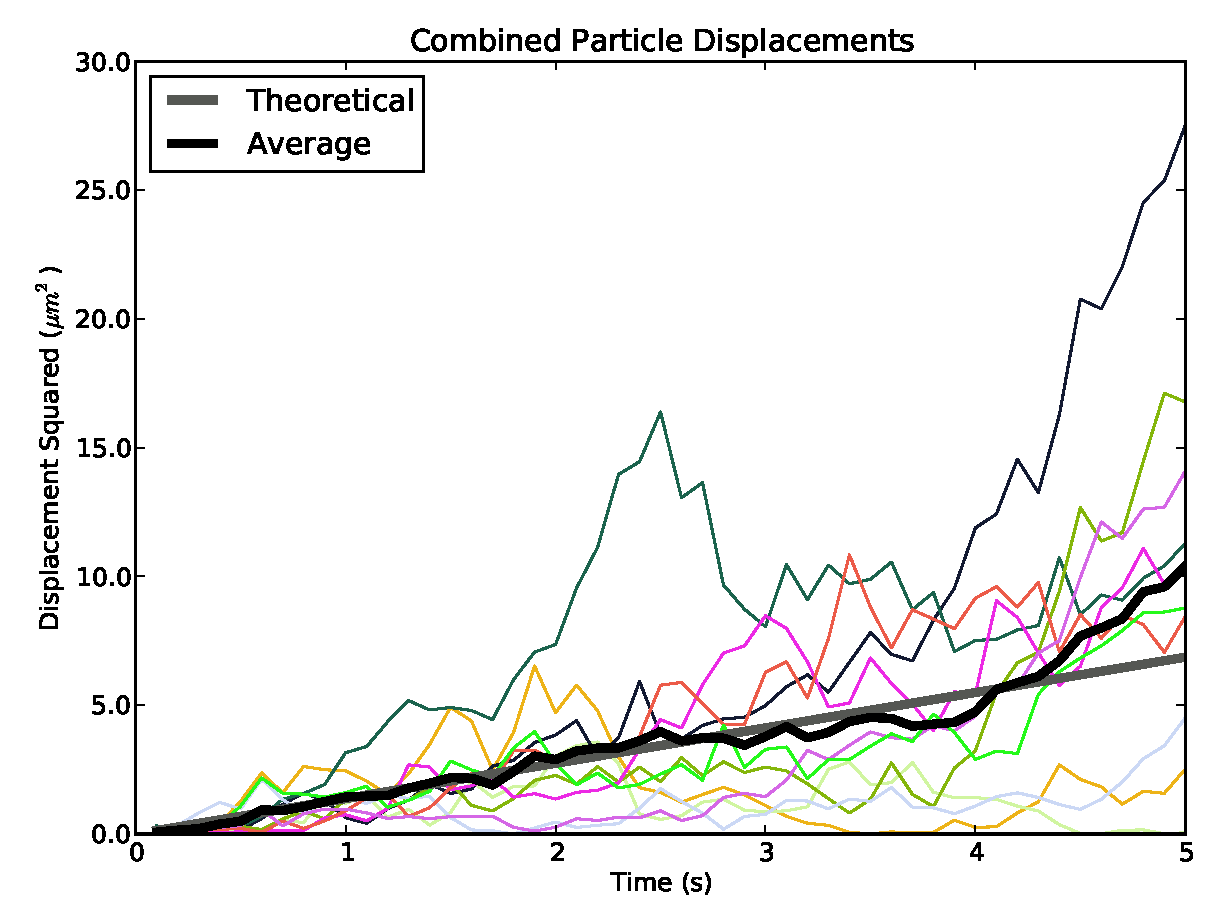
\includegraphics[width=\textwidth]{figures/many_particles_dispsq.pdf}
    \end{minipage}
    \begin{minipage}[t]{0.485\textwidth}
        \centering
        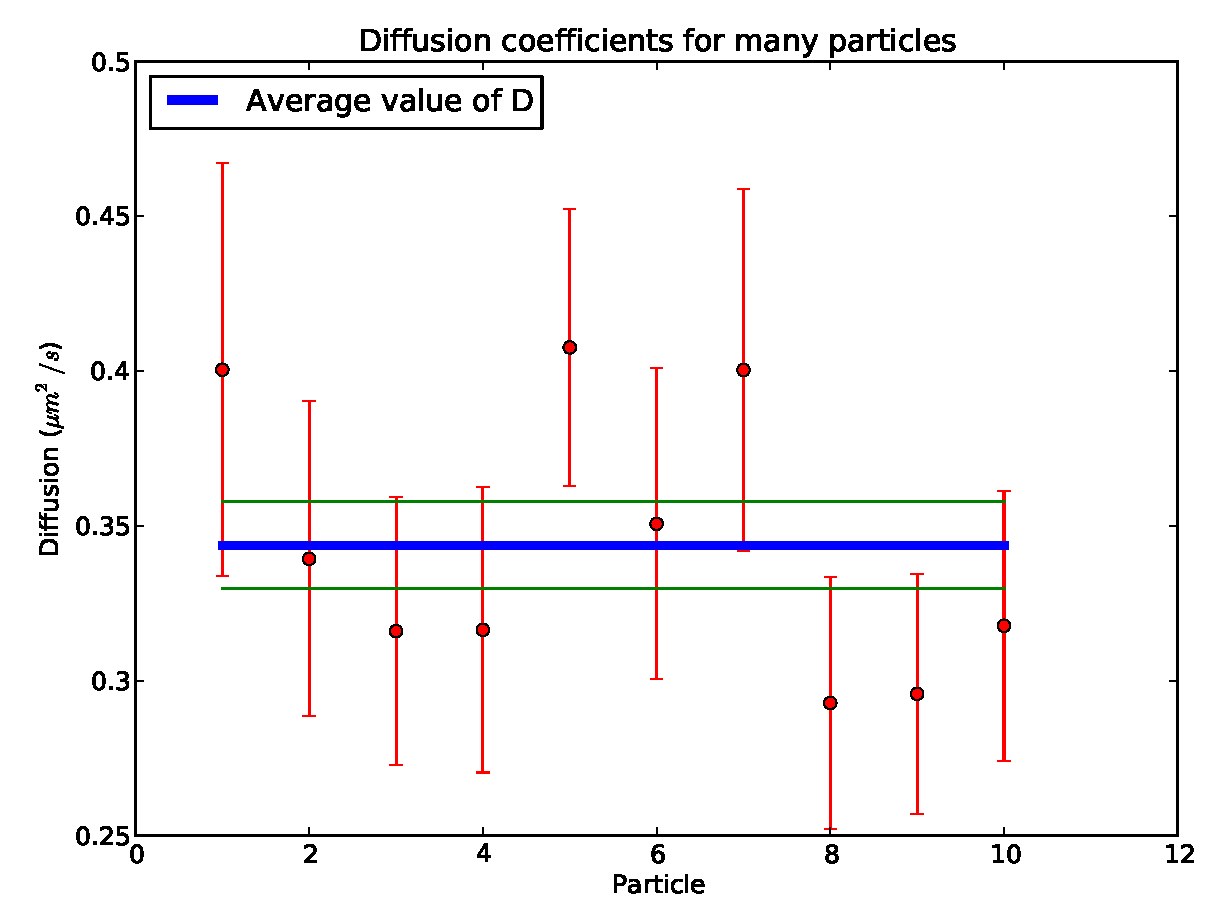
\includegraphics[width=\textwidth]{figures/many_particles_coef.pdf}
    \end{minipage}
    \caption{Monte Carlo simulation for a many particle system. The radius of
    the particles were half a micron and the viscosity of the solution for this
    simulation was 2.50 cP. This simulation matches the experimental conditions
    used to measure Brownian motion. The blue line on the right plot is the
    average of the diffusion coefficients and the green is the uncertainty on
    that average.}
    \label{many_particles_sim}
\end{figure}

% Particles undergoing bulk flow.
\begin{figure}
    \centering
    \begin{minipage}[t]{0.485\textwidth}
        \centering
        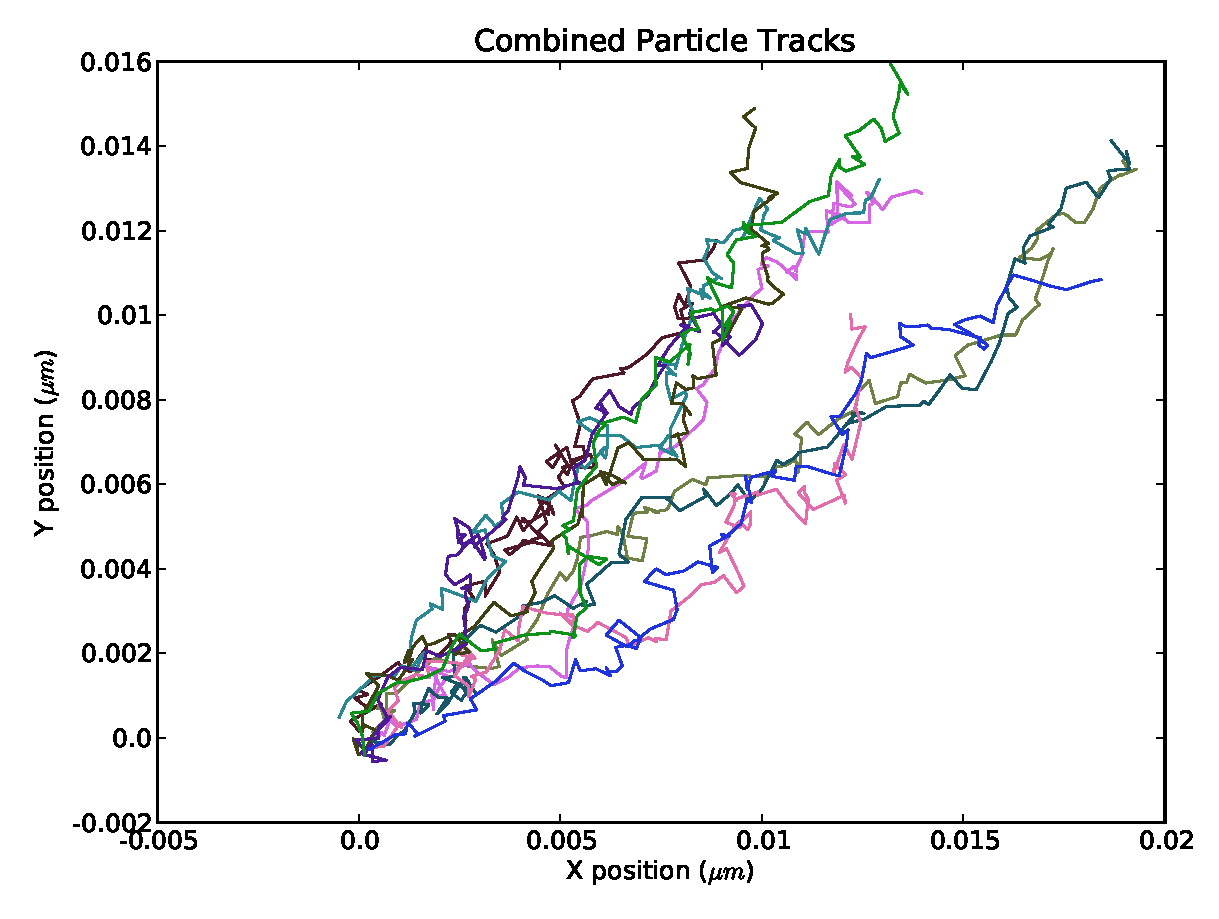
\includegraphics[width=\textwidth]{figures/mpbulk_track.pdf}
    \end{minipage}
    \begin{minipage}[t]{0.485\textwidth}
        \centering
        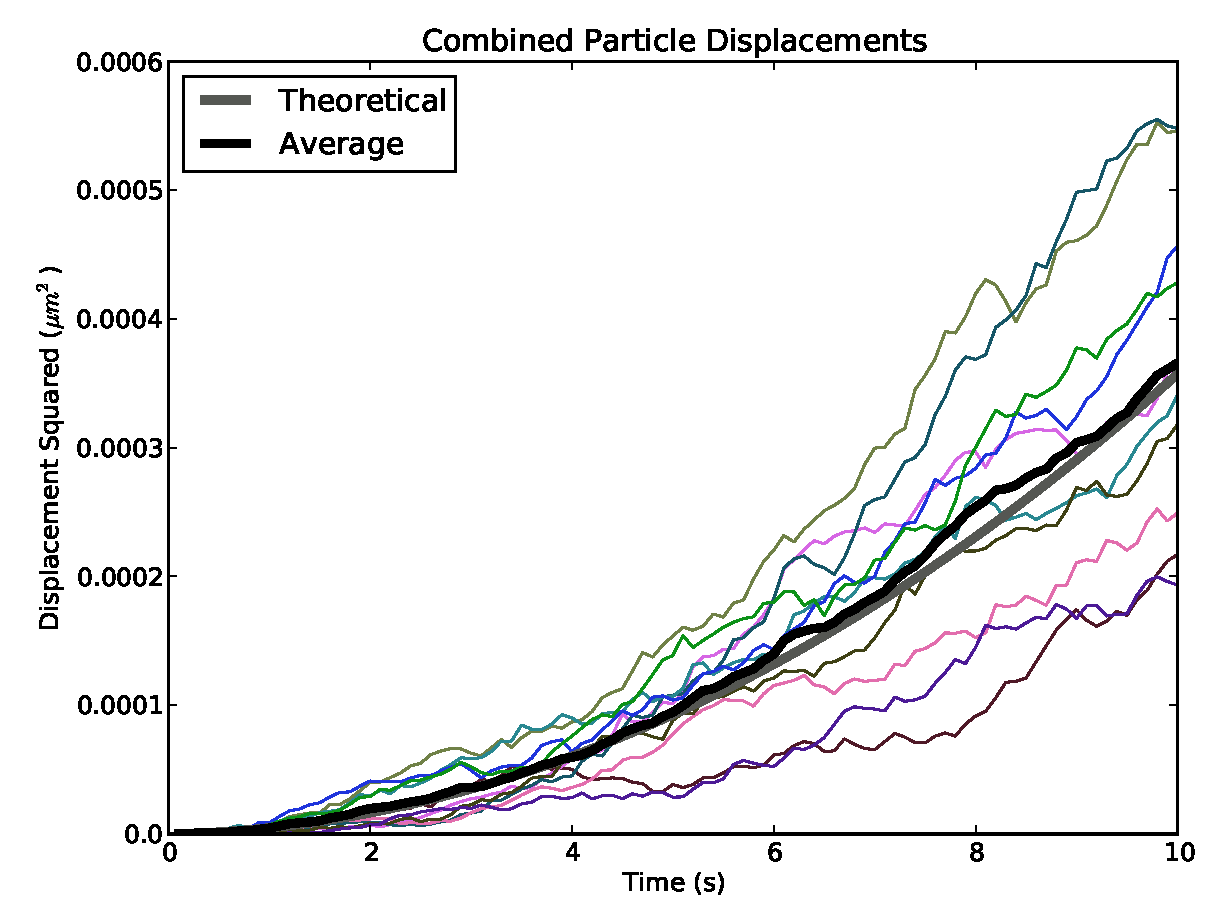
\includegraphics[width=\textwidth]{figures/mpbulk_dispsq.pdf}
    \end{minipage}
    \caption{Monte Carlo simulation for a many particle system undergoing a bulk
    flow. The system is the same as the system in
    Figure~\ref{many_particles_sim}, except that an extra flow with with
    velocity $\vec{v} = \sqrt{\frac{D}{2\Delta t}}
    \left(\hat{x} + \hat{y}\right)$ was added to the system.}
    \label{mpbulk_sim}
\end{figure}

\subsection{Bulk flow}

So far, it has been assumed that diffusion has been the only mechanism to
transport particles through a medium. This is not true in general. One example
of a transport mechanism for particles in a fluid is a constant bulk flow.
Adding bulk flow to the simulations is pretty straightforward. Consider a
displacement $\Delta \vec{r}$. This displacement can be written as a sum of two
mechanisms as
\begin{equation}
    \Delta \vec{r} = \Delta \vec{r_b} + \vec{v} \Delta t
    \label{bulk_disp}
\end{equation}
where $\Delta \vec{r_b}$ is the displacement due to Brownian motion and
$\vec{v}$ is a constant flow of the solution containing the particles. When
taking the average of \eqref{bulk_disp}, the term for $\vec{r_b}$ vanishes,
since it is Gaussian distributed and the average displacement then becomes
\begin{equation}
    \langle \Delta \vec{r} \rangle = \vec{v} \Delta t
\end{equation}
This provides a simple mechanism for determining from data whether particles are
being transported by a bulk flow by computing the vector components of the
flow.\\

Bulk flow can easily be added to the Monte Carlo simulations for Brownian
Motion. The variance of \eqref{desolution} defines the length scale of the
simulation to be $\sqrt{2D\Delta t}$. The bulk flow can be added to the
simulation as a scaling factor times the length scale, giving displacements as
\begin{equation}
    \Delta \vec{r} = \Delta \vec{r_b} + \vec{\epsilon} \sqrt{2D\Delta t}
    \label{bulk_disp_sim}
\end{equation}
where $\vec{\epsilon}$ is the scaling parameter that determines the strength of
the bulk flow in each direction. Clearly, it can be seen that the theoretical
velocity of the flow that drives the Monte Carlo is
\begin{equation}
    \vec{v} = \vec{\epsilon} \sqrt{\frac{2D}{\Delta t}}
\end{equation}
and the simulations can be used to see if the flow velocity can be extracted
from data. Another prediction that can be added to the Monte Carlo model is how
the total displacement squared will behave. Squaring \eqref{bulk_disp} and
taking the average gives
\begin{equation}
    \langle \Delta r^2 \rangle = \langle \Delta r_b^2 \rangle + v^2 \tau^2
    = 2dD\tau + v^2 \tau^2
    \label{bulk_flow_model}
\end{equation}
which has an extra quadratic term that vanishes in the absence of bulk flow.
This prediction can be seen in Figure~\ref{mpbulk_sim}. It should be noted that
Figures \ref{many_particles_sim} and \ref{mpbulk_sim} outline another method of
determining the diffusion coefficient and the bulk flow of a system. This can be
done by computing the average displacement squared at each point in time and
fitting to either a linear or quadratic fit. When applying the fitting to find
the bulk flow, only the magnitude of the flow can be found. The direction of the
flow has to be found by averaging the individual displacements.

\section{Experimental setup}

% OUTLINE
% 1. Explain microscope and techniques
%   i. Brightfield / Kohler
%   ii. Darkfield
% 2. Explain data collection methods.
%   i. Computer / visual studio
% 3. Particle tracking

Both of the experiments performed essentially use the same method of tracking
particles in a sample. How it works is that a microscope is plugged into a
computer, and software is used to track the particles and save data. Once the
data is saved, it is then analyzed to find certain quantities of interest and
their uncertainties.

\subsection{The Microscope}

\begin{SCfigure}
    \centering
    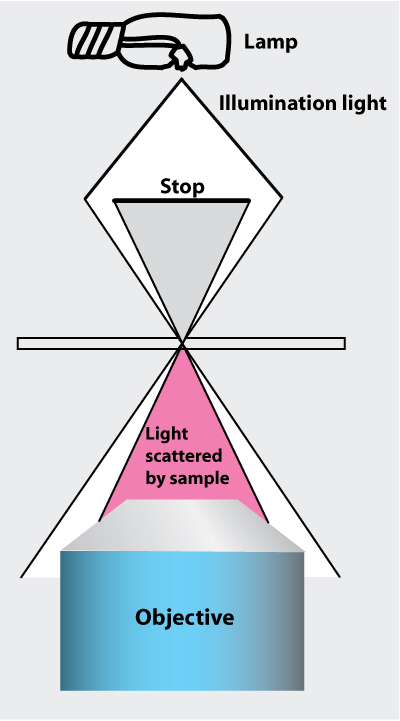
\includegraphics[width=0.3\textwidth]{figures/darkfield.jpg}
    \caption{Schematic diagram of dark-field illumination \cite{LabExp}. The
    stop creates an optical system where light is sent to the side of the sample
    and gets scattered off of it. This makes it possible for objects smaller
    than a wavelength of light that cannot be observed using bright-field
    illumination to be observable.}
    \label{darkfield}
\end{SCfigure}

The microscope used for tracking the particles was the Zeiss Axiovert 200. This
microscope was used for both bright-field and dark-field microscopy.
Bright-field microscopy is used to observe light that is reflected off of
objects, whereas dark-field microscopy is done by scattering light off of
particles. Bright-field microscopy was not very useful in the context of the
experiments performed in this lab since the size of the particles tracked with
the microscope were about the size of wavelengths of visible light. Fortunately,
dark-field microscopy makes it possible to observe tiny objects in the
microscope samples. An illustration of the basic principle behind dark-field
illumination can be seen in Figure~\ref{darkfield} \cite{LabExp}. This technique
makes it possible to observe tiny particles that are not visible by reflecting
light.\\

Before setting up dark-field illumination, K\"{o}hler illumination must be first
achieved. This also must be done when changing the objective on the microscope.
The reason for this is that setting up K\"{o}hler illumination creates an
illumination on a sample that is very uniform \cite{KohlerWiki}. Setting up
K\"{o}hler illumination is fairly straightforward. This is done by closing the
iris a small amount and adjusting the position of the iris until the center of
the iris can be viewed from the eyepiece. This step is repeated until the iris
is almost closed entirely and the entire open region of the iris is centered
with respect to the view of the eyepiece. Once the iris is centered, the iris is
then opened so that the edge of the iris is outside of the field of view. After
this is done, the microscope can then be set to use dark-field illumination. An
example of a sample being viewed with dark-field illumination can be seen in
Figure~\ref{darkfieldsphere}.

\begin{figure}
    \centering
    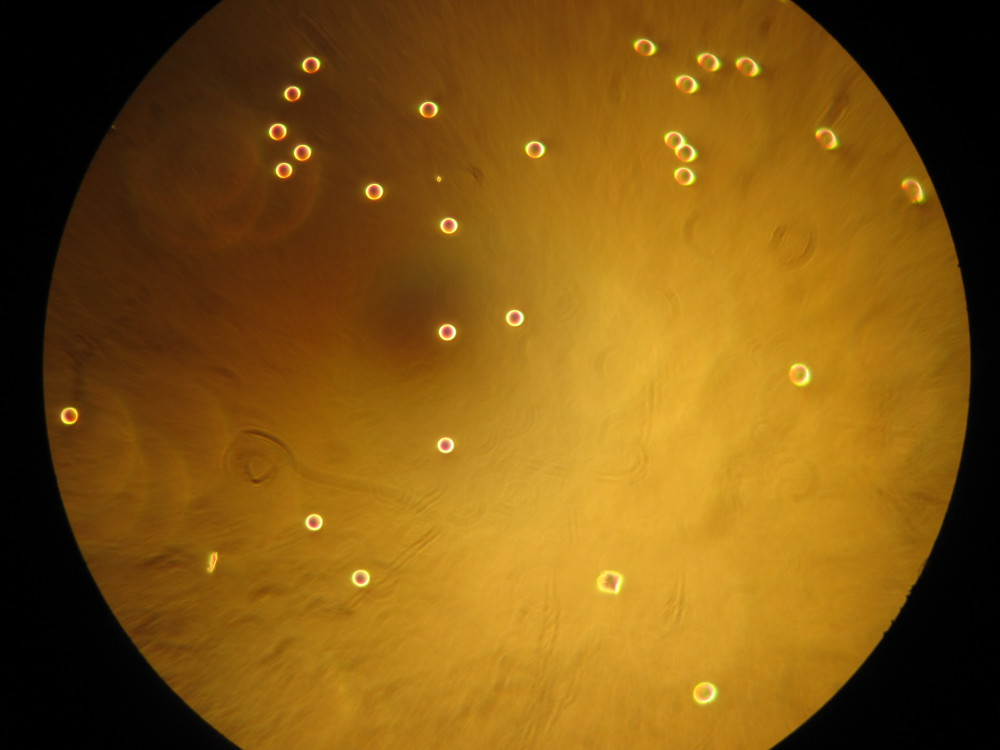
\includegraphics[width=0.6\textwidth]{figures/IMG_0029.JPG}
    \caption{Polystyrene spheres under the microscope viewed using dark-field
    illumination.}
    \label{darkfieldsphere}
\end{figure}

\subsection{Particle Tracking}

In order to measure the diffusion using \eqref{diffusion_data}, the particles in
the field of view of the microscope must be tracked. Particle tracking has two
main components, blob finding and tracking. Once the trajectories of the
particles have been recorded, then statistics can be run on them to compute the
diffusion coefficient and its uncertainty \cite{LabSoftware}. The particles were
tracked using software that was unfortunately written in the C\# language.\\

Blob finding is the method of locating particles. This is done by computing the
background level of an image by taking the mean brightness and flagging all
spots in the image that exceed a certain brightness. The brightness level that
determines whether or not a spot is a particle is called the Z-score threshold,
and that sets the number of standard deviations above the background a spot must
be in order for it to be considered a particle \cite{LabSoftware}. Of course, in
order for a set of pixels to be considered a particle, they must fall within a
limit set by the user of the tracking software that dictates the pixel range
that a particle can be.\\

The method described so far has one giant deficiency. Suppose there are static
structures, cell walls for example, in the microscope camera's field of view
that are much brighter than the objects that are moving. If that happens, it is
likely that the moving objects will not be distinguishable from background
noise. Additionally, the large static structures would probably be tracked, and
that would ruin a set of data being used to compute the diffusion of a system or
detect active transport methods occurring in a cell.\\

Before computing the mean of a frame to find the background, the average image
must be subtracted from the frame to remove noise and static structures like
cell walls. The easiest way to do this would be to collect a movie of data
frames, take the average of all frames, subtract that average from each frame,
and then run the particle tracking algorithm. Unfortunately, this method is
undesirable because it cannot run in real time. Fortunately, there is a way to
get a real-time average, and that is done with exponential smoothing.
Exponential smoothing is defined as such \cite{ExpSmoothWiki}
\begin{equation}
    \begin{array}{rcl}
        s_0 & = & x_0 \\
        s_j & = & \alpha x_j + \left(1-\alpha\right) s_{j-1},
    \end{array}
\end{equation}
where $s_j$ is the average images up to iteration $j$, $x_j$ is the camera image
recorded at iteration $j$, and $\alpha$ is the smoothing parameter, where
$0 < \alpha < 1$. By default, exponential smoothing was not implemented in the
source code for the tracking software, but adding it was easy to do in only 2
lines of code. The smoothing factor that was used was chosen to be 0.05.\\

In addition to exponential smoothing, another feature that needed to be added to
the particle tracking software was an algorithm to find the center of the blobs.
Originally, the tracking software used the brightest pixel in a blob as the
center. However, for oddly shaped blobs, that will be inaccurate. This can be
fixed by using a method analogous to finding the center of mass of a massive
object. The center of brightness for a 2-D object is defined as
\begin{equation}
    \vec{R}_{CB} = \frac{\int \vec{r} \rho\left(x,y\right) dA}
    {\int \rho\left(x,y\right) dA}
\end{equation}
where $\rho \left(x,y\right)$ is the density of brightness of each point in an
image. Of course, when dealing with images from a camera, the integrals turn
into sums, since the camera images are discrete.\\

Blob finding is not sufficient to track particles because it does not address
whether or not a blob in one frame and a blob in the next frame are the same
blob. The simplest way to track particles is to use the nearest neighbor method,
which matches particles in one frame to the closest particles in the next frame.
While this method is very simple, it only works when particles are loosely
packed together and are not moving very fast. Another method to do is create
groups of particles and connect particle tracks based on that. All of the
particle tracking functionality in the tracking software was already implemented
and didn't need to be changed in any way.\\

Finally, the software must be calibrated so that it can properly convert
distances in pixels to distances in meters. This is done by viewing particles of
known size in the microscope and measuring how many pixels wide they are for
each magnification setting in the tracking software. The conversion factors for
each magnification can be seen in the following table.

\begin{center}
    \begin{tabular}{| c | c | c |}
        \hline
        10x & 20x & 40x\\
        \hline
        0.666 $\mu m / px$ & 0.4 $\mu m / px$ & 0.222 $\mu m / px$ \\
        \hline
    \end{tabular}
\end{center}

\section{Brownian Motion of Micro-Spheres}

% Outline
% 1. Explain how to

Einstein's theory of Brownian motion can be tested by tracking spherical
particles in a solvent. If Einstein's theory is true, then the data should
support the model in \eqref{diffusion_data} where the diffusion coefficient is
defined as \eqref{diffusion_def}. In order to properly test Einstein's theory,
particles of a variety of sizes must be placed in solvents of varying viscosity.
This experiment tests Einstein's theory with polystyrene spheres of diameters
0.47 $\mu m$ and 1.0 $\mu m$ in solvents of viscosities 1.66 cP, 2.50 cP, and
4.65 cP. The solvents used are glycerol and PVP. The following table shows the
values of the diffusion coefficient predicted by \eqref{diffusion_def} at
$20\ ^{\circ}\text{C}$.

\begin{center}
    \begin{tabular}{| c | c | c | c |}
        \hline
        Diameter & 1.66 cP & 2.50 cP & 4.65 cP \\
        \hline
        0.47 $\mu m$ &
            $1.00 \times 10^{-12} \ \text{m}^2 / \text{s}$ &
            $7.31 \times 10^{-12} \ \text{m}^2 / \text{s}$ &
            $3.93 \times 10^{-12} \ \text{m}^2 / \text{s}$ \\
        \hline
        1.0 $\mu m$ &
            $5.17 \times 10^{-13} \ \text{m}^2 / \text{s}$ &
            $3.43 \times 10^{-13} \ \text{m}^2 / \text{s}$ &
            $1.84 \times 10^{-13} \ \text{m}^2 / \text{s}$ \\
        \hline
    \end{tabular}
\end{center}

% Polystyrene spheres in solvents
\begin{figure}
    \centering
    \begin{minipage}[t]{0.485\textwidth}
        \centering
        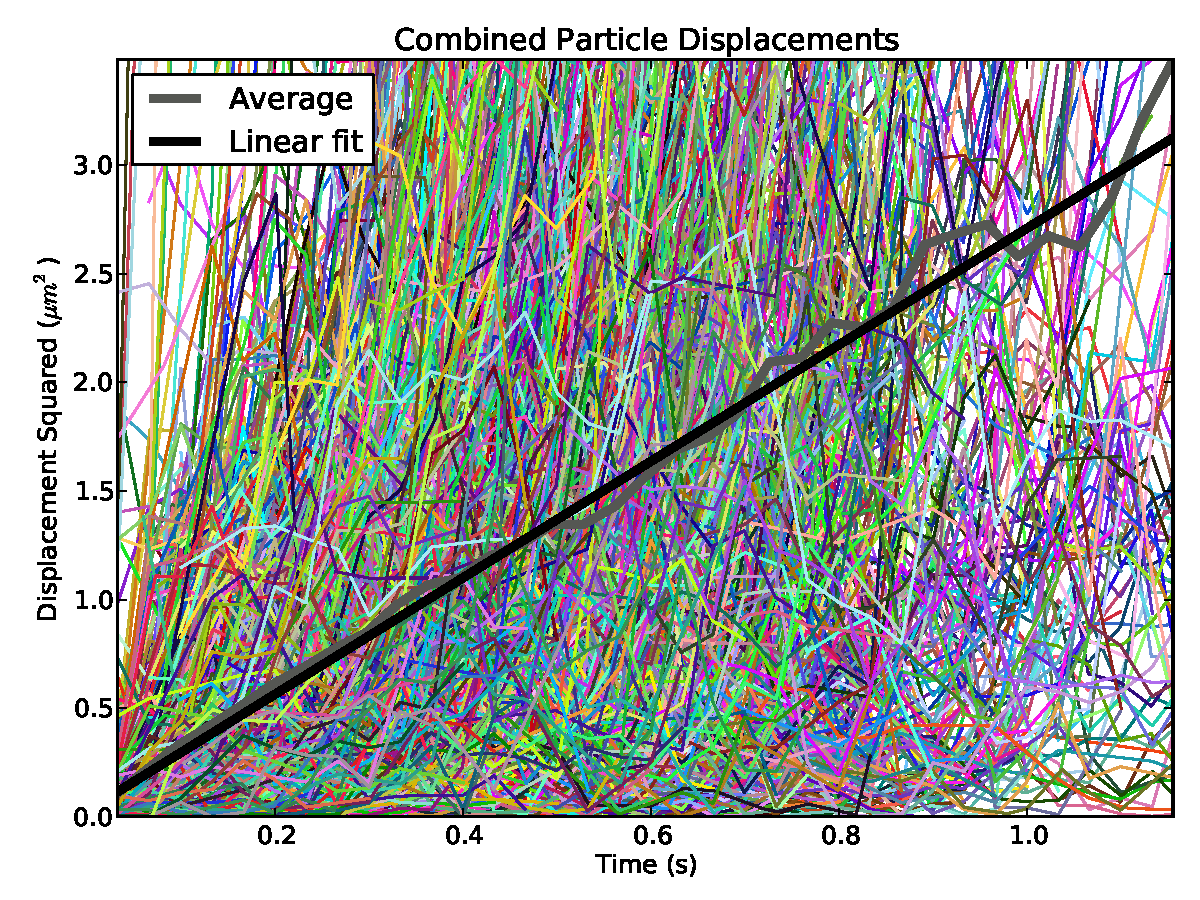
\includegraphics[width=\textwidth]{figures/d047_v250_G_1.pdf}
    \end{minipage}
    \begin{minipage}[t]{0.485\textwidth}
        \centering
        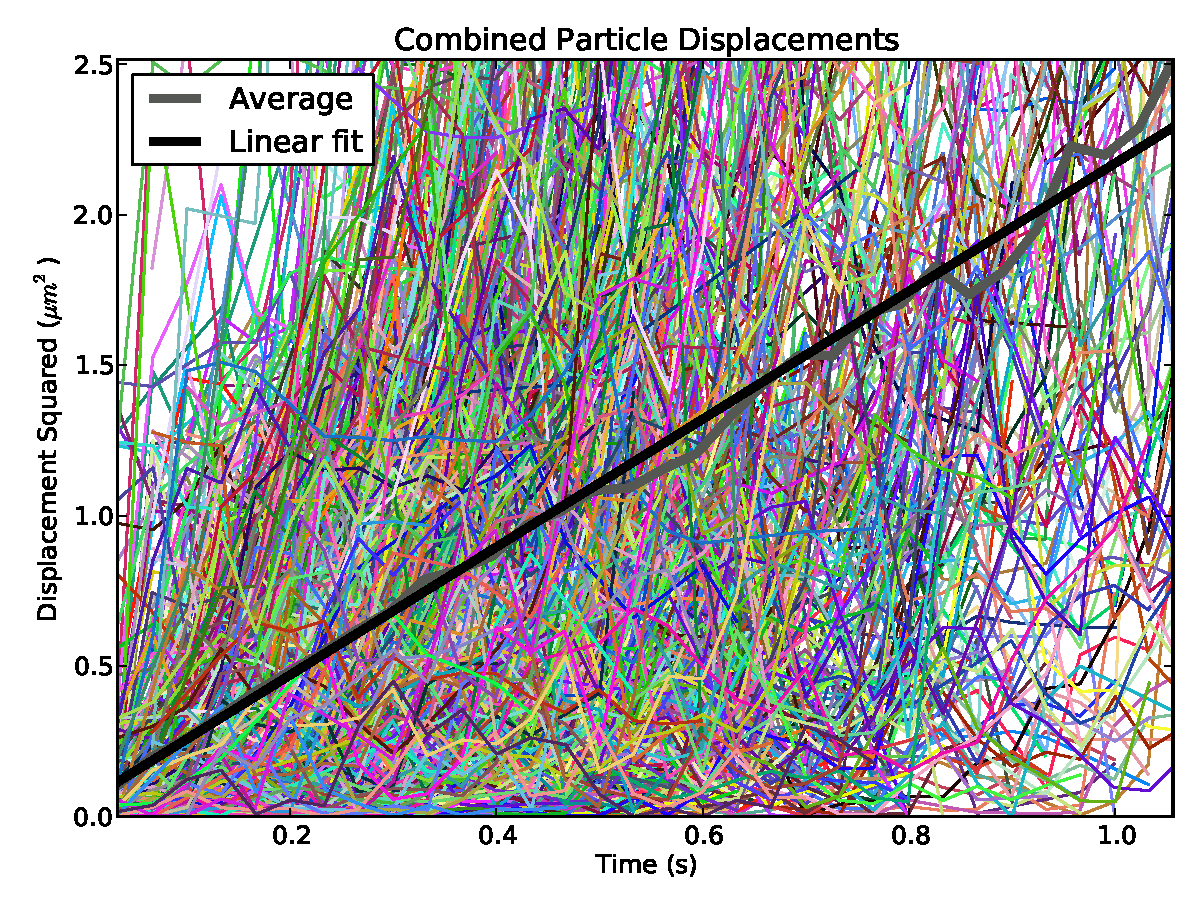
\includegraphics[width=\textwidth]{figures/d047_v250_P_1.pdf}
    \end{minipage}
    \caption{(left) Polystyrene spheres in glycerol solvent. (right) Polystyrene
    spheres in PVP solvent. Both plots are for spheres with diameters of 0.47
    $\mu m$ and the viscosity of both solvents used is 2.50 cP.}
    \label{polysphere}
\end{figure}
\ \\

% TODO I think I probably need another paragraph, but there really isn't too
% much to say about the polystyrene spheres.

The diffusion coefficient can be computed two ways. The first is to directly use
Einstein's relation for 2 dimensions
\begin{equation}
    \langle \Delta r^2 \rangle = 4D \tau
    \label{fit2d}
\end{equation}
to compute a value of the diffusion coefficient for each track and then take the
weighted mean over all tracks of these values of $D$ and get the diffusion
coefficient that way. Another way to calculate $D$ is to use \eqref{fit2d} and
fit the average net displacement at each point in time and compute $D$ from the
slope of the linear fit. In the averaging method, the error on the diffusion
coefficient computed for each track is the standard deviation of the
displacements divided by the square root of the number of steps recorded for
that track. Due to the limitations of the tracking software, the number of
recorded steps is not the same for each particle track. The weighted mean
diffusion, and its uncertainty are therefore
\begin{equation}
    \begin{aligned}
        \langle D \rangle & = &
            \sigma^2_{\langle D \rangle}
            \sum\limits_{i=1}^N
            \frac{\langle D_i \rangle}{\sigma^2_{\langle D_i \rangle}} \\
        \frac{1}{\sigma^2_{\langle D \rangle}} & = &
            \sum\limits_{i=1}^N \frac{1}{\sigma^2_{\langle D_i \rangle}} \\
    \end{aligned}
\end{equation}
where $\sigma_{\langle D \rangle} = \sigma_{D_i} / \sqrt{n_i}$. When finding
the diffusion coefficient using a linear fit, the uncertainty on the diffusion
can be obtained from the covariance matrix of the fit. Each system measured had
at least two data recordings, and the results of each method of getting the
diffusion coefficient can be combined in a weighted average for each method
separately. The following tables show the values of the diffusion coefficients
and their uncertainties, calculated from averaging displacements and creating a
linear fit. Unless otherwise noted, the solvent is glycerol. It should be noted
that the curve fitting method produces results must closer to the theoretical
value calculated with \eqref{diffusion_def}.\\

Diameter: 0.47 $\mu m$\\
\begin{tabular}{| c | c | c | c | c |}
    \hline
    Averaging method & 1.66 cP & 2.50 cP & 4.65 cP & 2.50 cP (PVP) \\
    \hline
    Diffusion coefficient ($\mu m^2 / s$) &
        0.613 &
        0.424 &
        0.275 &
        0.378 \\
    \hline
    Uncertainty &
        $3 \times 10^{-3}$ &
        $2 \times 10^{-3}$ &
        $1 \times 10^{-3}$ &
        $2 \times 10^{-3}$ \\
    \hline
\end{tabular}

\ \\
\ \\
\begin{tabular}{| c | c | c | c | c |}
    \hline
    Curve fitting method & 1.66 cP & 2.50 cP & 4.65 cP & 2.50 cP (PVP) \\
    \hline
    Diffusion coefficient ($\mu m^2 / s$) &
        1.014 &
        0.645 &
        0.434 &
        0.526 \\
    \hline
    Uncertainty &
        $8 \times 10^{-3}$ &
        $5 \times 10^{-3}$ &
        $4 \times 10^{-3}$ &
        $4 \times 10^{-3}$ \\
    \hline
\end{tabular}

\ \\
\ \\
Diameter: 1.0 $\mu m$\\
\begin{tabular}{| c | c | c | c | c |}
    \hline
    Averaging method & 1.66 cP & 2.50 cP & 4.65 cP & 2.50 cP (PVP) \\
    \hline
    Diffusion coefficient ($\mu m^2 / s$) &
        0.395 &
        0.386 &
        0.252 &
        0.482 \\
    \hline
    Uncertainty &
        $2 \times 10^{-3}$ &
        $2 \times 10^{-3}$ &
        $1 \times 10^{-3}$ &
        $3 \times 10^{-3}$ \\
    \hline
\end{tabular}

\ \\
\ \\
\begin{tabular}{| c | c | c | c | c |}
    \hline
    Curve fitting method & 1.66 cP & 2.50 cP & 4.65 cP & 2.50 cP (PVP) \\
    \hline
    Diffusion coefficient ($\mu m^2 / s$) &
        0.566 &
        0.592 &
        0.342 &
        0.659 \\
    \hline
    Uncertainty &
        $3 \times 10^{-3}$ &
        $4 \times 10^{-3}$ &
        $5 \times 10^{-3}$ &
        $7 \times 10^{-3}$ \\
    \hline
\end{tabular}

\ \\
% TODO answer more lab questions

\section{Intracellular Movement in Onion Cells}

\begin{figure}
    \centering
    \begin{minipage}[t]{0.485\textwidth}
        \centering
        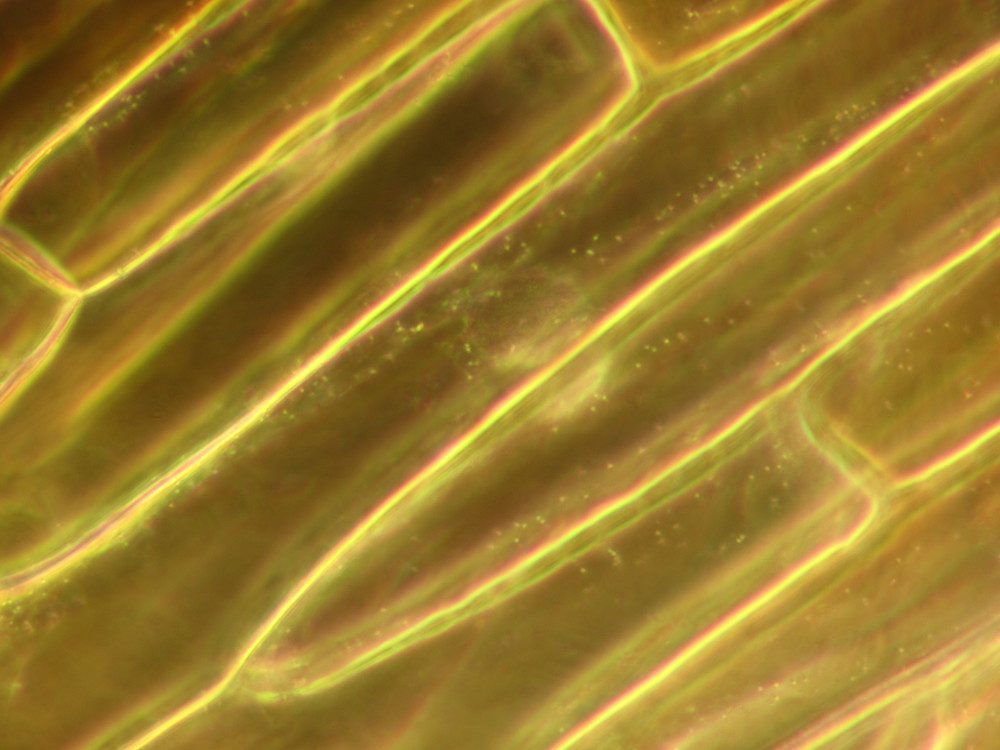
\includegraphics[width=\textwidth]{figures/IMG_0049.JPG}
        \caption{Vesicles moving along transport paths in red onion cells.}
        \label{onionphoto}
    \end{minipage}
    \begin{minipage}[t]{0.485\textwidth}
        \centering
        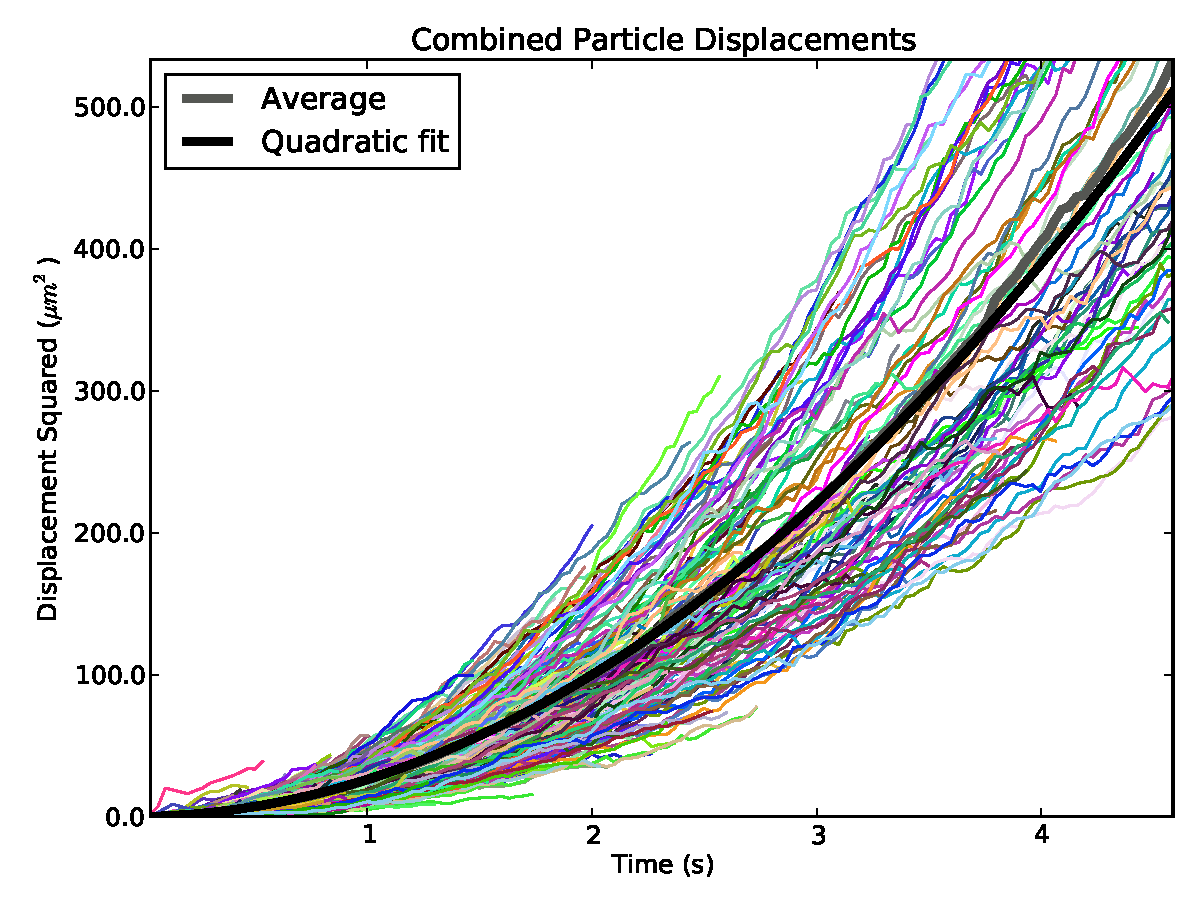
\includegraphics[width=\textwidth]{figures/bulk_onion.pdf}
        \caption{Vesicles in the onion cell undergoing bulk flow. The flow in
        this sample was very large, and it could be the result of saline flowing
        to the edge of the slide.}
        \label{bulk_onion}
    \end{minipage}
\end{figure}

The organelle used by cells to transport material is called a vesicle. In the
low Reynold's number limit, the amount of work that it takes to transport a
vesicle from one part of a cell to another can be computed from Stokes' Law
\cite{StokesLawWiki}
\begin{equation}
    F_d = 6\pi \eta r v
\end{equation}
where $F_d$ is the drag force on the particle and $v$ is the velocity of the
particle. Using the definition of the diffusion coefficient
\eqref{diffusion_def}, it can be shown that the work to transport a particle a
small distance is
\begin{equation}
    dW = 2v \frac{k_B T}{D}dr
\end{equation}
This can be computed for each step in a particle track and then summed to get
the total work. Since this work is the amount of work needed to resist the drag
of the intracellular fluids, this work can come from diffusion or active
transport. It should be noted that diffusion is insufficient as a transport
mechanism. One reason for this is because diffusion produces random walks for
vesicle trajectories, whereas vesicles are often transported along non-random
trajectories (see Figure~\ref{onionphoto}).\\

The techniques used to calculate the diffusion coefficients of the systems with
the polystyrene spheres can be used to calculate the diffusion coefficient of
the cells, and therefore calculate the viscosity of the cytosol. The diameter of
the particles detected in the tracking software was about 4 pixels, which
corresponds to 900 nm. By tracking the vesicles in regions where the only motion
is Brownian motion, it was found that the diffusion coefficient for the cells
was $0.700(5) \mu m^2 / s$, which implies that the viscosity of the cytosol is
about 1.38 cP.\\

% Combined particle tracks.
\begin{figure}
    \centering
    \begin{minipage}[t]{0.485\textwidth}
        \centering
        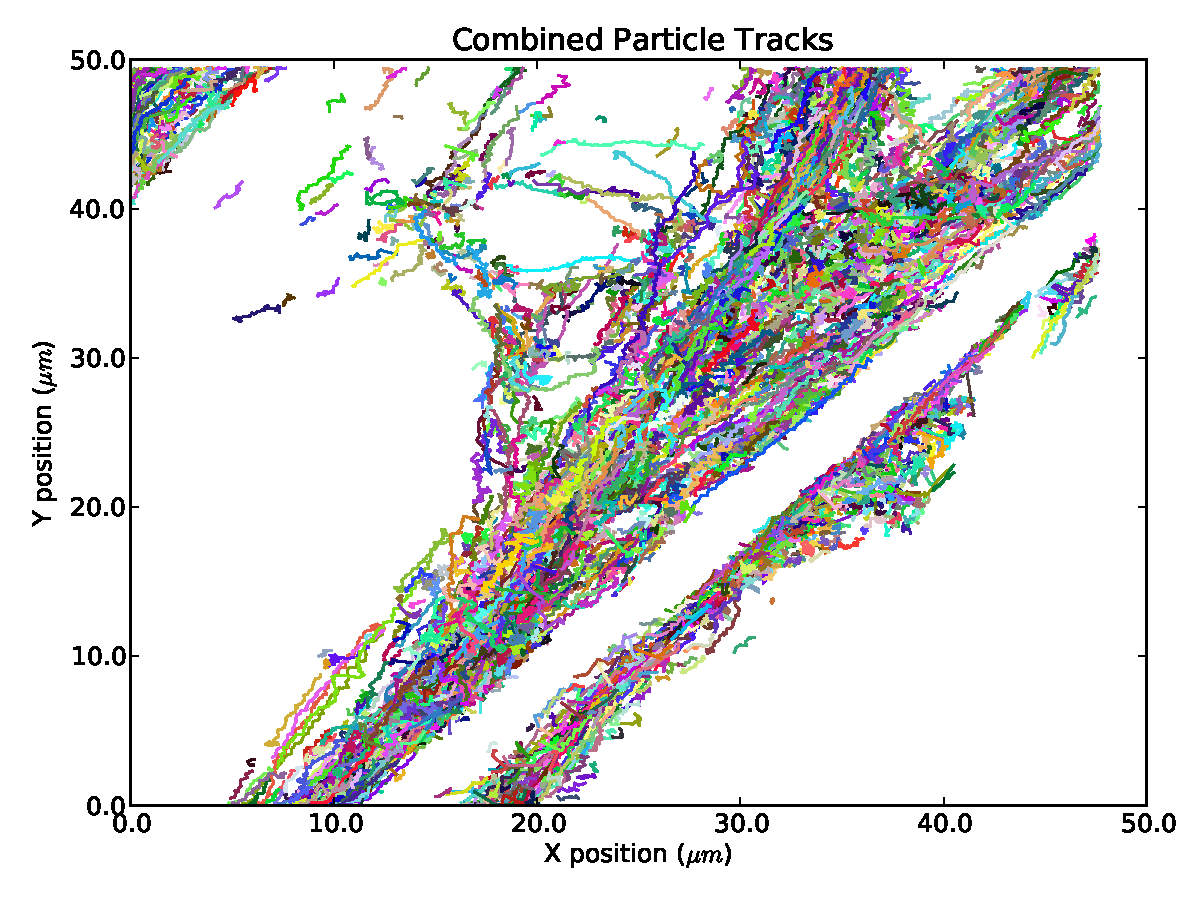
\includegraphics[width=\textwidth]{figures/red_onion_test_17_tracks.pdf}
    \end{minipage}
    \begin{minipage}[t]{0.485\textwidth}
        \centering
        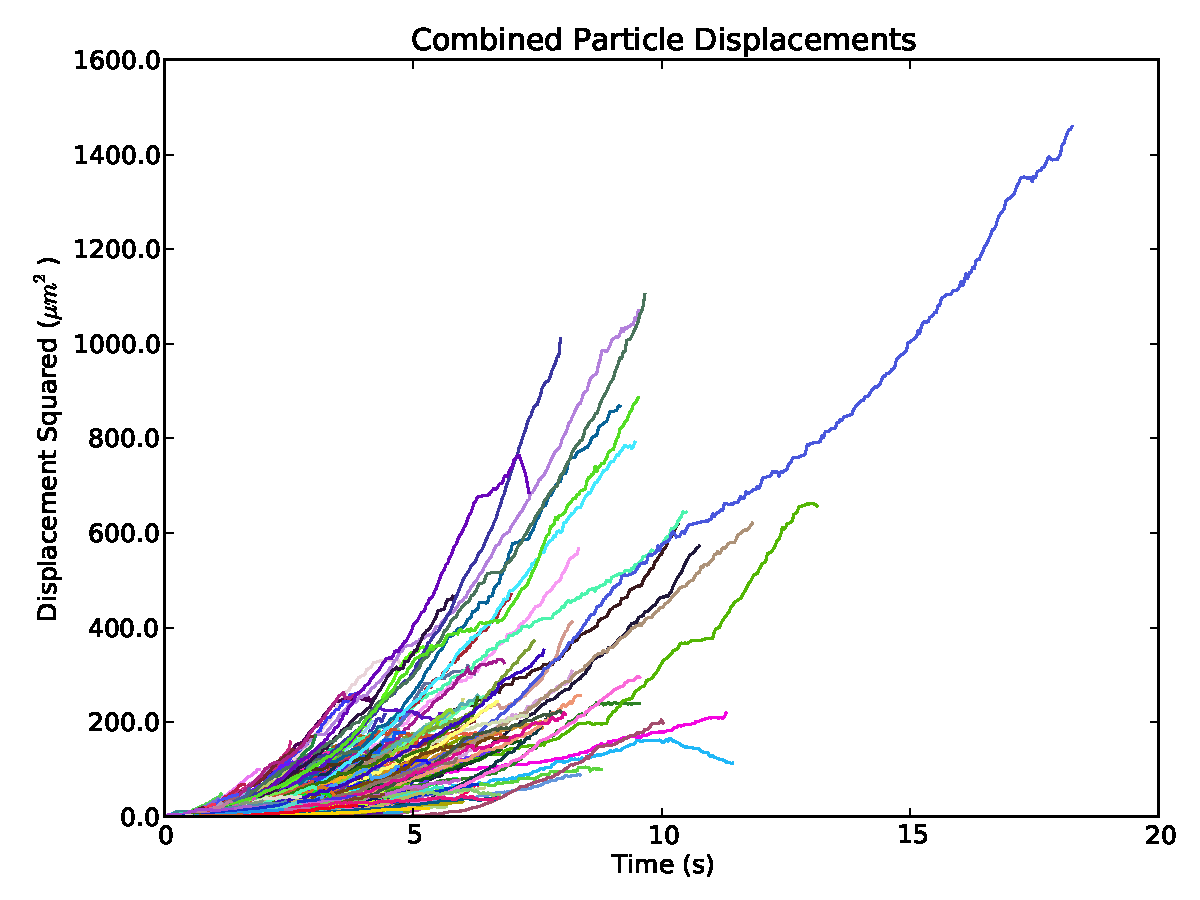
\includegraphics[width=\textwidth]{figures/red_onion_test_17_dispsq.pdf}
    \end{minipage}
    \caption{Transport paths and displacements of vesicles in a red onion cell.}
    \label{onion_tracks}
\end{figure}

\begin{figure}
    \centering
    \begin{minipage}[t]{0.485\textwidth}
        \centering
        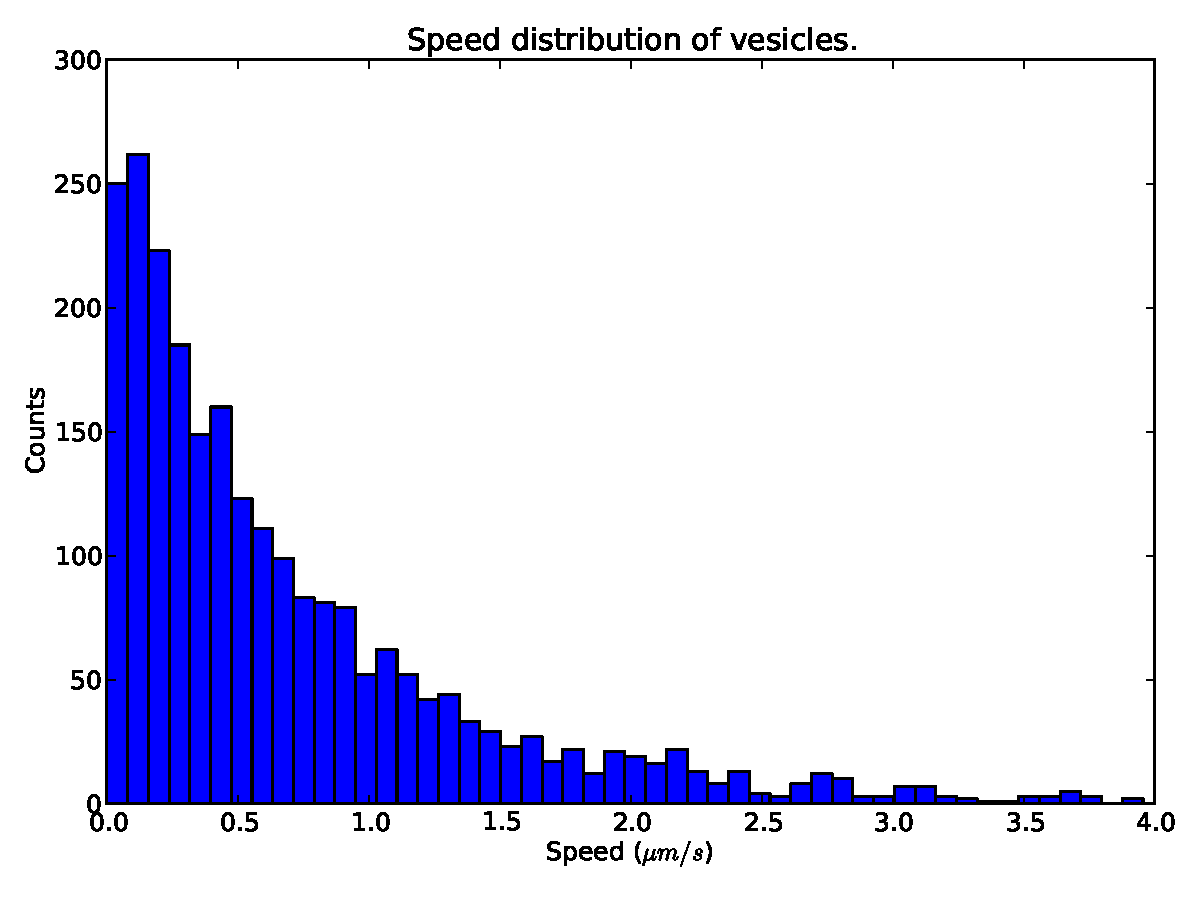
\includegraphics[width=\textwidth]{figures/red_onion_test_17_speeds.pdf}
        \caption{The speed distribution of particles has an exponential drop off
            rate.}
        \label{speed_dist}
    \end{minipage}
    \begin{minipage}[t]{0.485\textwidth}
        \centering
        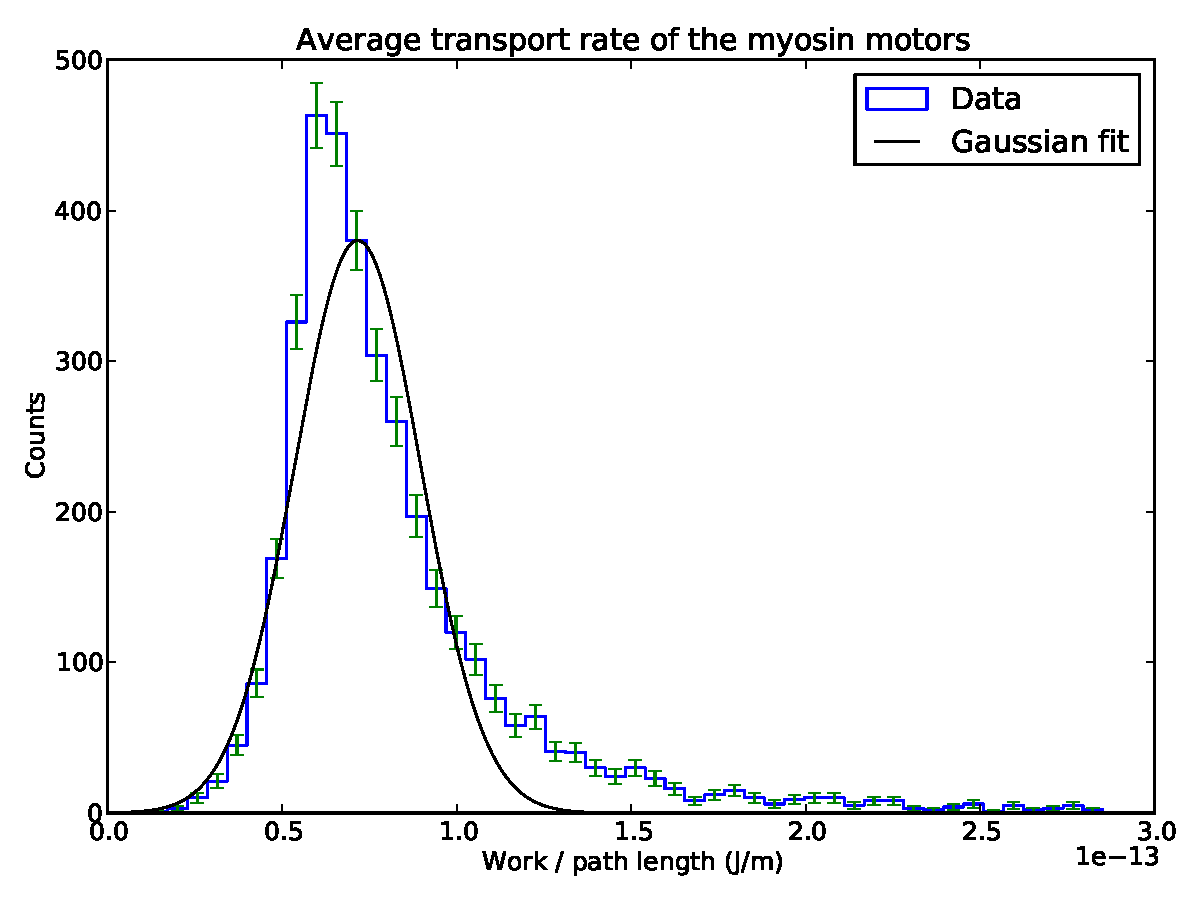
\includegraphics[width=\textwidth]{figures/red_onion_test_17_workrate.pdf}
        \caption{The work required to transport each vesicle is something that
            is fairly straightforward to calculate. However, since each particle
            traverses a different trajectory, a more interesting quantity is the
            work that it takes to transport a vesicle normalized to the line
            integral of the vesicle's trajectory. This produces a somewhat
            sharply peaked distribution that behaves like a Gaussian.}
        \label{work_rate}
    \end{minipage}
\end{figure}

The combined particle tracks for vesicles in a red onion can be seen in
Figure~\ref{onion_tracks}. It is clear from this that there are pathways of
cellular transport. This can both be seen from the left figure of the particle
tracks, which shows the trajectories, as well as the right figure, which shows a
tracks having quadratic displacement, as predicted by \eqref{bulk_flow_model}.
Another verification of \eqref{bulk_flow_model} can be seen in
Figure~\ref{bulk_onion}. In that figure, there was a strong flow of solution
moving the vesicles. One possible causes of that system was saline flowing to
the edge of the slide.\\

In addition to the particle tracks and overall displacements, the speed
distribution of the vesicles undergoing active transport is something that
should be looked at (see Figure~\ref{speed_dist}). Most vesicles are not moving
very quickly, as the drop off in the speed distribution is exponential. In all
of the regions measured that contained active transport, the RMS speed was
fairly consistent, and the combined average of the RMS speed was
$1.13(2)\ \mu m/s$.\\

The measurements of active transport can be used to quantify the amount of
molecular motors it takes for certain cellular processes to occur. Stokes' Law
can be used to calculate the amount of work that it takes to transport particles
over a distance. Since each vesicle travels a different length, the average
amount of energy per unit length traveled to transport a vesicle can be found by
normalizing the work for transporting each vesicle with the line integral of
each vesicle's trajectory. The distribution of the total work per total path
length can be seen in Figure~\ref{work_rate}. The mean of the Gaussian fit of
that distribution was fairly consistent over all transport regions, and the
combined average of it was $7.64(5) \times 10^{-14}\ \text{J/m}$. Additionally,
the combined average amount of work done on a vesicle was found to be
$3.55(2) \times 10^{-19}$ J.\\

The theory behind cellular transport is that myosin motors are a driver of
active transport \cite{Motors}. The process of a myosin motor cycle converts one
molecule from ATP to ADP. This, along with the energy release from converting
ATP to ADP and the efficiency of the myosin motors can be used to find the
approximate number of motors involved in intracellular transport. The energy of
an ATP to ADP reaction is 20.5 kJ/mol \cite{ATPADP}, and the energy for a single
reaction can be found by dividing that number by Avogadro's constant. The peak
efficiency of the myosin motors is about 0.4 \cite{Myosin}. This information,
plus the average amount of work done on a vesicle can be used to conclude that
it cellular transport takes about 26,000 myosin cycles.\\

% Brownian motion figures for onions can go here for now.
\begin{figure}
    \centering
    \begin{minipage}[t]{0.485\textwidth}
        \centering
        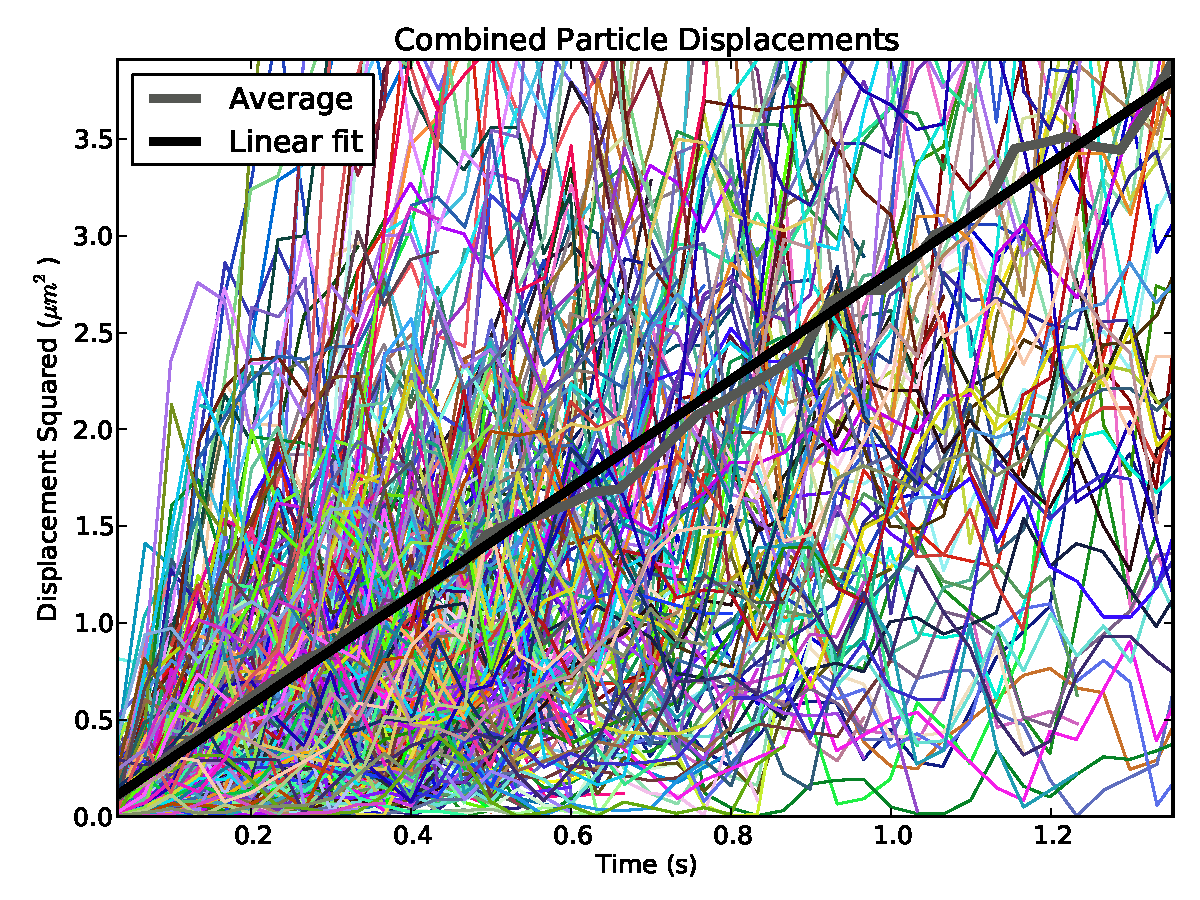
\includegraphics[width=\textwidth]{figures/red_onion_test_4.pdf}
    \end{minipage}
    \begin{minipage}[t]{0.485\textwidth}
        \centering
        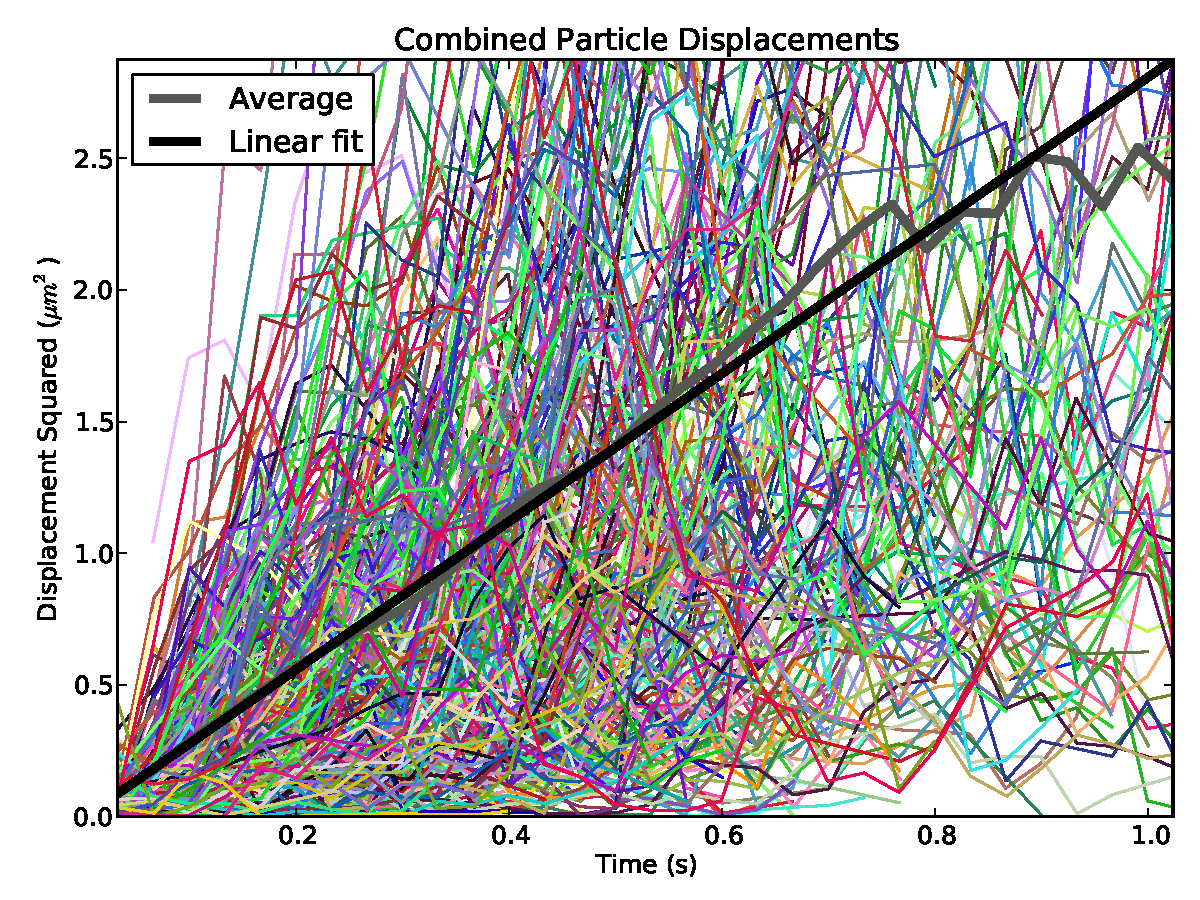
\includegraphics[width=\textwidth]{figures/red_onion_test_5.pdf}
    \end{minipage}
    \caption{Brownian motion results from onion cells. The diffusion coefficient
    computed from these two plots implies that the viscosity of the cytosol is
    about 1.38 cP.}
    \label{onion_brownian}
\end{figure}

The source code written for the simulations and analysis has been uploaded to
Github and can be found at \cite{Bitbucket}\\
https://bitbucket.org/domagalski/physics111-advanced-lab/.

\newpage
\bibliographystyle{unsrt}
\bibliography{reference_list}{}

\end{document}
